Over the years, indexes have been widely used in databases to improve the speed of data retrieval. In the past decades, the database indexes generally fall into the hand-engineered data structures, such as B-Tree, KD-Tree, etc. These indexes have played a crucial role in databases and have been used widely in modern data management systems (DBMS) such as PostgreSQL. Despite their huge success, a shortcoming of these data structures is the lack of consideration of how the database records distributed. We use an example to demonstrate how distributions can affect the efficiency of database indexes.

\begin{mscexample}
	For example, if the dataset contains integers from $1$ to $1$ million, then the keys can be used directly as offsets. With the keys used as offsets, the value with a given key can be retrieved in $\mathcal{O}(1)$ time complexity while B-Tree requires $\mathcal{O}(\log n)$ time complexity for the same query. From the perspective of space complexity, we do not need any extra overhead by using the key as an offset directly, while the B-Tree needs extra $\mathcal{O}(n)$ space complexity to save the tree.
\end{mscexample}

From the above example, we found that there are two promising advantages of leveraging the distribution of the data:
\begin{enumerate}
  \item It may be faster when performing queries, especially when the number of entries in the database are rather huge.
  \item It may take less memory space, as we only need to save the model with constant size.
  \end{enumerate}

Nowadays, to learn the distribution and apply it to database indexes, Tim Kraska et al. proposed learned indexes \cite{kraska2018case}, \cite{li2020lisa}, where machine learning techniques are applied to automatically learn the distribution of the database entries and build the data-driven indexes. In this project, we implemented both hand-engineered indexes and the learned index. After that, we explore the possibilities of using convolutional neural networks as database indexes. This report is organised into the following chapters:

\begin{enumerate}
	\item \textbf{Introduction}. In this chapter, we illustrate the organisation of this report and introduce the general information about database indexes.
	\item \textbf{Implementation}. In this chapter, we present our implementation of the B-Tree for 1-D data and $K$D-Tree for 2-D data. We also present our implementation of the learned index for 1-D data \cite{kraska2018case} and 2-D data \cite{li2020lisa}. This includes a baseline learned index, a recursive model and all components of LISA framework. 
	\item \textbf{Evaluation}. In this chapter, we report evaluation of our implementation. 
	\item \textbf{Insights and Findings}. We demonstrate our findings in this chapter. Besides, we also discuss the advantages and disadvantages of different indexes.
	\item \textbf{Convolution and CNN for Learned Indexes}. In this chapter we explore the possibilities of using convolution operation and convolutional neural network to build learned indexes.
	\item \textbf{Conclusions}. 
\end{enumerate}

\section{Notations}

In this report, we will use the following notations:

\begin{table}[h]
\begin{tabularx}{\textwidth}{@{}XX@{}}
\toprule
  \underline{Sets and Spaces} \\
  $\mathbb{R}$ & The set of real numbers \\
  $\mathbb{R}^d$ & The set of $d$ dimensional real space \\
  \underline{Random Variables} \\
  $\boldsymbol{X}$ & A vector or matrix \\
  $x$ & A single value in $\textbf{X}$ \\
  $(x,y)$ & A tuple contains two values \\	
  \underline{Hyper-Parameters} \\
  N   & A pre-set hyper parameter \\
  \underline{Functions} \\
  $\mathcal{LR}$ & Linear Regression Function\\
  $\mathcal{P}$ & Polynomial Function\\
  $\mathcal{M}$ & Mapping Function\\
  $\mathcal{O}$ & Big-O notation for complexity\\
  $\mathcal{SP}$ & Shard Prediction Function\\
  $\mathcal{Q}$ & Range Query \\
  $\mathcal{K}$ & $K$NN Query \\
  \underline{Others} \\
  $\clubsuit$ & End of Example \\
  $\blacksquare$ & End of Proof \\
\bottomrule
\end{tabularx}
\end{table}


\section{Terminologies}

In the following chapters, we will use the following terminologies

\textbf{Index model} is a function that maps the index of a row of data into the location (e.g. page index) of the data. For example, in one-dimensional case, the index models include B-Tree, Linear Regression models, etc.

\textbf{Key} is a special attribute in the database that could identify a record. In our work, the key could be a scalar in one-dimensional case, or a $(x,y)$ pair in two-dimensional case.

\textbf{Order of a tree} is the maximum number of children that a node can have.

\textbf{Internal node} is any node of a tree that has child nodes and is not a root node.

\textbf{Leaf node} is any node that does not have child nodes.

\textbf{Level} of a node is defined as the number of edges between this node and the root node.


\section{Assumptions}

\begin{figure}[!htb]
\centering
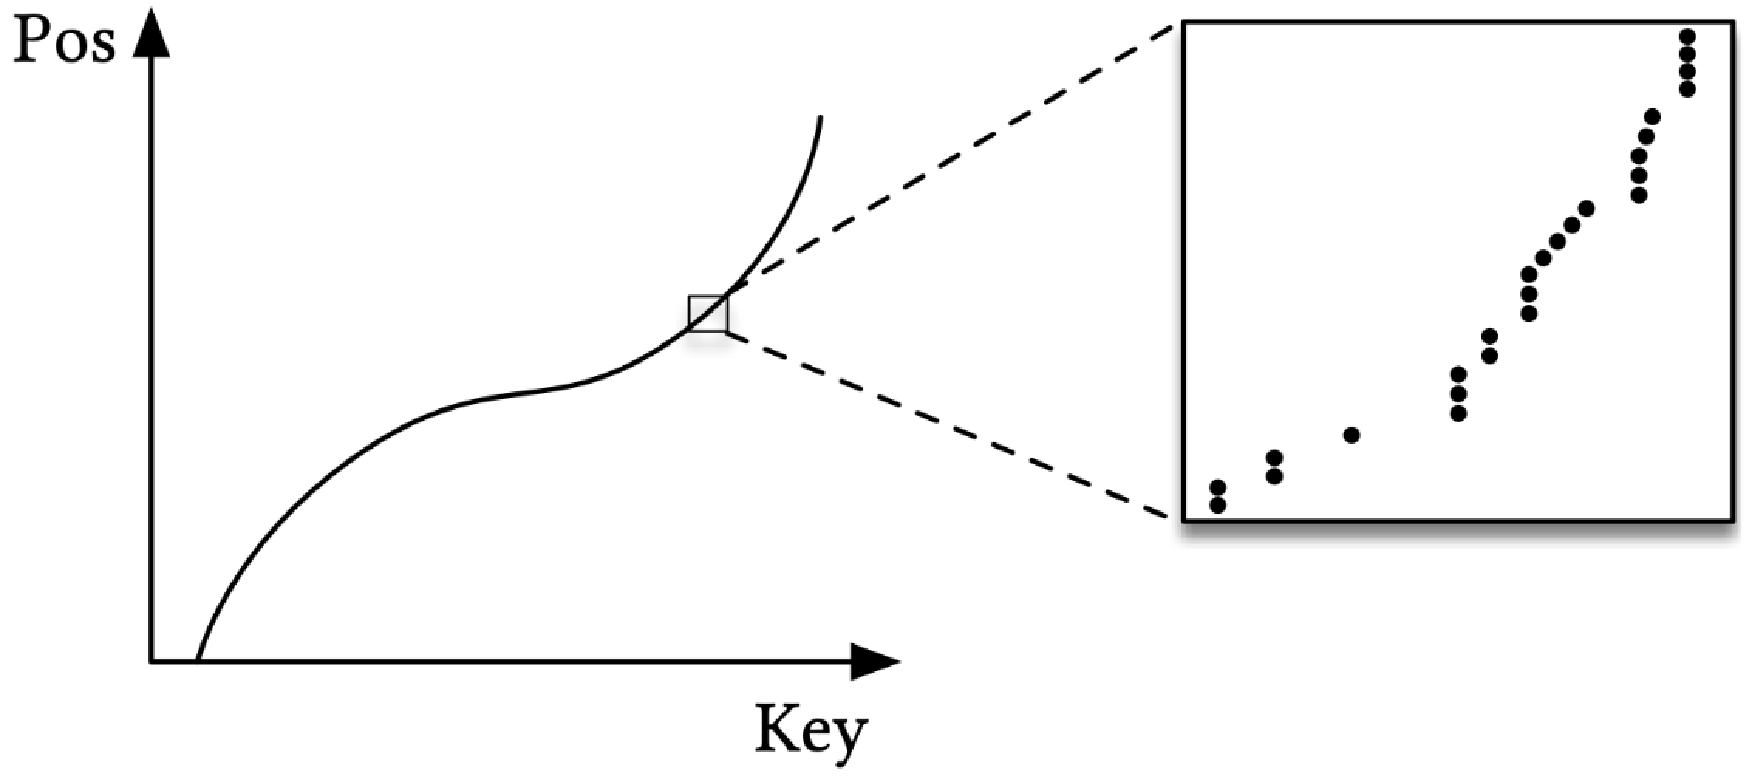
\includegraphics[width=0.8\textwidth]{graphs/introduction/cdf_assumptions}
\caption{The illustration of indexes as CDFs, originally from \cite{kraska2018case}}
\label{fig:indexes_as_cdf}
\end{figure}


Formally, we define the index of each record as $x$ and the corresponding location as $y$ and we represent the whole data as $(X, Y)$ pairs with the total number of pairs defined as $N$. We could then normalise the $Y$ into $\tilde{Y}\in[0,1]$ so that the $\tilde{y}$ represents the portion of the $y$ among the whole $Y$. With these definitions, we can then define a function $F:X\to \tilde{Y}$ that maps the index into the portion of the $y$. We have $y=F(x)* N$. As the output of this function can be considered as the probability of $X\leq x$, we can regard this function $F(x)$ as the cumulative distribution function (CDF) of $X$, i.e. $F(x)=\mathbb{P}(X\leq x)$. Now that $N$ is determined by the length of data records, we only need to learn such CDF and we called the learned CDF function as \textbf{learned index model}.

In Fig. \ref{fig:indexes_as_cdf}, we illustrate the relationship between the key and its position. The raw keys and their positions are illustrated in the zoomed-in view and the zoomed-out view presents a shape of the relation. In this figure, we present why the position can be regarded as a CDF: the position of a key is always the position of previous key plus $1$, i.e. the position describes how many keys are there before a certain key $x$. If we divide it by the total number of keys, we will have the result as the possibility of how many keys are smaller than the certain key $x$, i.e. $\mathbb{P}(X\leq x)$. The result is therefore the CDF of $X$.

\begin{mscexample}
	From the perspective of the distribution of data records, our previous example can be rephrased as following. Our data records are $(X, Y)$ pairs with a linear relation, i.e. $y=x, \forall y\in Y$. We are looking for a function $F$ such that $y=x=F(x)* N$, and hence we end up with $F(x)=\frac{1}{N}*x$. If we use this linear function $F(x)$ as the index model, then we could locate the data within $\mathcal{O}(1)$ time complexity and we only need to store the total number of records as the only parameter. Compared with B-Tree whose query complexity is $\mathcal{O}(\log n)$, the potential of using learned index to handle huge amount of data is enormous. 
\end{mscexample}

In order to ensure the learned index model to be the desired CDF, we need to make the following assumptions:

\begin{enumerate}
	\item All data records are stored statically. Hence we do not take insertion and deletion into consideration. If there is some insertion or deletion, then the total size of the data records, $N$, will be different. Therefore, if insertion or deletion are involved, we cannot calculate the position as we show above.
	\item All data records are sorted according to theirs keys $\boldsymbol{X}$. Only when the data records are sorted according to the keys, we can regard the index model as CDF, i.e. $F(x)=\mathbb{P}(X\leq x)$.
	\item For simplicity, we assume that our data records are stored in a continuous memory space. In other words, the indices of pages in this project is continuous integers and all the data records are loaded into memory.
\end{enumerate}


